\chapter{Metodología de trabajo}
\label{chap:Metodologia de trabajo}
\Abstract{Para poder desarrollar w innovar es necesario primero definir una estructura base sobre la que edificar. Y se debe determinar un plan a seguir que sirva de guía.}

\section{Motivación}
\label{chap:Metodología sec:Motivación}
La industria avanza a un ritmo constante y cada día es más necesario la implantación de sistemas robóticos para poder llevar a cabo tareas que los humanos no podemos desarrollar o que presentan una elevada tasa de errores humanos o tienen un elevado nivel de peligrosidad. Al dotar a estos sistemas de inteligencia y un sistema de visión artificial, se consigue que se pueda adaptar mejor al entorno y se evite tener que re-programar los robots con cada cambio de las condiciones de operación. Avanzamos hacia una sociedad en la que los robots serán la principal mano de obra y para llegar a ese objetivo es necesario invertir y desarrollar más los sistemas actuales. Por ello se ha propuesto como proyecto la integración de un sistema de visión artificial en un robot industrial. Con este proyecto se podrá modernizar las instalaciones del Grupo Antolín\textsuperscript{\textregistered} y aumentar las capacidades de la línea de montaje y ensamblaje actual.

\section{Objetivos}
\label{chap:Metodología sec:Objetivos}
Este trabajo parte de un proyecto actualmente en desarrollo con un sistema de visión artificial ya desarrollado e implantado. Desgraciadamente la implantación actual presenta limitaciones así como una tasa de error superior a los requisitos planteados por el Grupo Antolín.

Para poder superar las limitaciones actuales se ha planteado el desarrollo de un nuevo sistema que debe de mejorar las capacidades de identificación y detección de las piezas así como poder determinar el punto de agarre óptimo. El sistema debe de ser modular de forma que se pueda adaptar fácilmente a nuevas piezas. Y con el fin de que el robot tenga la mayor posibilidad de coger la pieza, también se debe de determinar el vector normal al punto de agarre. Por último, se pide que sea independiente del resto del proyecto de forma que pueda ser fácilmente manejado, modificado y actualizado.

Con el fin de cumplir dichos requisitos se deben plantear unos objetivos de corto, medio y largo alcance a seguir durante todo el desarrollo del trabajo:

\begin{itemize}
	\item Desarrollo de una base de datos sintética:
	\begin{itemize}
		\item Investigación y prueba de diferentes sistemas/herramientas (bpi, zpi Zumo labs y Blenderproc).
		\item Obtención de primeras imágenes RGB y de profundidad.
		\item Obtención de imágenes de profundidad, mapa de normales, identificación de las piezas, mapas de segmentación, etc.
		\item Introducción de aleatoriedad y repetibilidad al sistema.
		\item Generación de un \textit{Pipeline} para la automatización del proceso.
		\item Introducción de ruido en las imágenes para mejorar la robustez.
	\end{itemize}
	\item Desarrollo de una base de datos real complementaria tanto para la fase de entrenamiento como evaluación del sistema.
	\item Desarrollo de las nuevas redes neuronales:
	\begin{itemize}
		\item Investigación y pruebas de diferentes sistemas/herramientas (YOLO, MobilNet, redes regresoras, etc).
		\item Planteamiento y definición de la estructura modular a desarrollar. Una primera red para la detección de piezas, seguida de una red para la detección de zonas de intereses con probabilidad de ser el punto de agarre óptimo. Y finalmente un una red neuronal del tipo regresor para la determinación del punto de agarre. 
		\item Primeros desarrollos independientes de las partes modulares del sistema
		\item Desarrollo y corroboración del conjunto modular
		\item Creación del sistema de evaluación tanto del conjunto como de las partes modulares del sistema
		\item Entrenamiento y evaluación de todo el sistema con diferentes configuraciones y bases de datos.
		\item Comparativa y determinación del sistema óptimo.
		\item Implantación del nuevo sistema de visión artificial
	\end{itemize}
\end{itemize}

\section{Arquitectura del sistema}
\label{chap:Metodología sec:Arquitectura}
El sistema se compone de tres elementos claves: un robot industrial para poder interactuar con las piezas, una cámara RGB-D para la captura de imágenes y Python para el procesamiento de las imágenes y la toma de decisiones. Es necesario que estos tres elementos funcionen correctamente y estén comunicados entre sí. La arquitectura básica se puede ver en \autoref{chap:Metodología fig:Arq1}

\begin{figure}[ht]
	\centering
	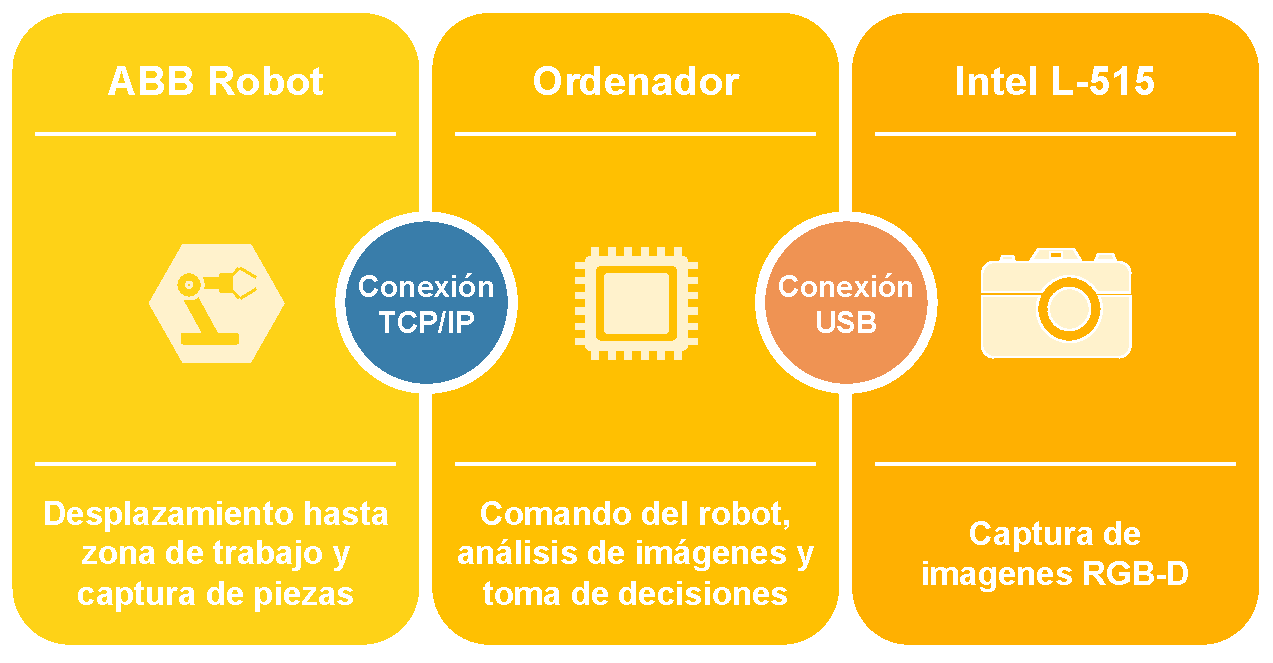
\includegraphics[width=0.9\textwidth]{Metodologia/Arquitectura.pdf}
	\caption{Esquema de la arquitectura del sistema}
	\label{chap:Metodología fig:Arq1}
	\vspace{-5pt}
\end{figure}

A continuación, se va a detallar todo el proceso desde el arranque del sistema hasta el final del mismo y se analizarán cada una de las etapas que constituyen el proceso. Este se puede ver gráficamente en \autoref{chap:Metodología fig:Arq2}. El sistema debe compenetrase con los sistemas actuales los cuales diseñan los pedidos que se deben de preparar y ensamblar. Estos pedidos se reciben y se procesan para establecer qué piezas se desean y en que orden deben de ser recogidas por medio de un proceso cíclico.

Una vez procesado el pedido y establecida la primera pieza a recoger se debe de desplazar el robot a la zona de trabajo y prepararse  para la captura de dicha pieza. Una vez reubicado el robot, un sistema de cámaras capturará la escena para determinar la posición de la pieza/piezas que se desean capturar frente a la posición del robot. Esta imagen es analizada por el sistema de visión artificial que se encargará de "en primera instancia" identificar las piezas para entre ellas poder centrarse solo en las que se desea capturar. A continuación, si se trata de una pieza de dimensiones grandes se analizará más en profundidad para determinar los posibles puntos de agarre. Y una vez determinados estos puntos de agarre un regresor determinará el centro exacto de dichos puntos de agarre así como el vector normal a dicho punto (dirección que debe emplear la muñeca del robot para capturar la pieza). Si por el contrario se trata de una pieza de dimensiones reducida se empleará el centro de la pieza como punto de agarre.

Esta información es transmitida al robot permitiéndole así poder capturar la pieza y depositarla en la cesta del pedido. Para ello este se deberá aproximar a la pieza seleccionada siguiendo en la medida de lo posible la trayectoria normal determinada. Al aproximarse a la pieza también deberá reducir la velocidad de operación para evitar colisionar.

\begin{figure}[ht]
	\centering
	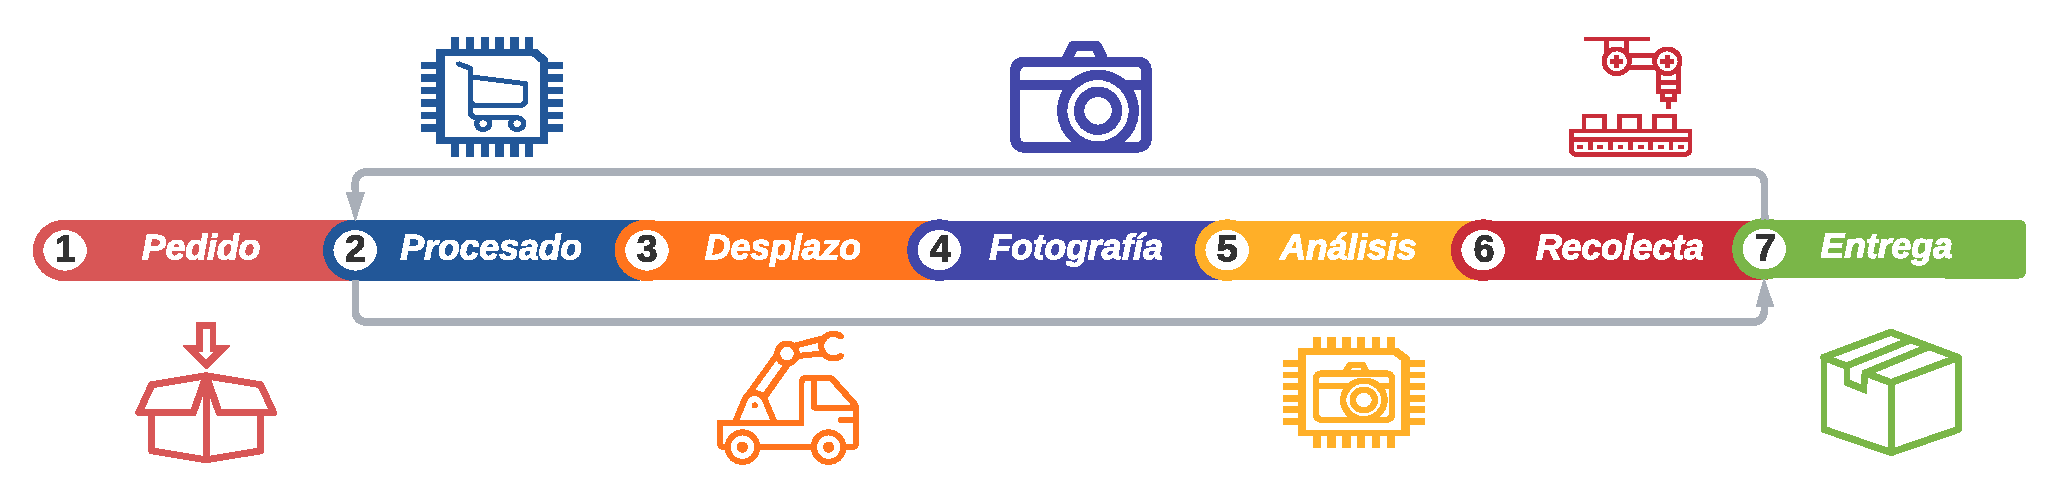
\includegraphics[width=1\textwidth]{Metodologia/Esquema arquitectura.pdf}
	\caption{Diagrama de las etapas del sistema}
	\label{chap:Metodología fig:Arq2}
	\vspace{-5pt}
\end{figure}

\section{Herramientas}
\label{chap:Metodología sec:Herramientas}
\begin{itemize}
	\item Cámara Intel RealSense L515 \cite{IntelL515} y Wrapper de Python para Intel Realsense \cite{SDK}.
	\item Ordenador con los siguientes SO/paquetes/programas:
		\begin{itemize}
			\item Ubuntu 20.04 LTS
			\item Blender 2.93.5
			\item BlenderProc 2.0 (Blender API)
			\item PyTorch 1.10.1
			\item Tensorflow 2.7.0
			\item CUDAToolkit
			\item Python 3.8 o superior
			\item Conda ó miniconda
		\end{itemize}
\end{itemize}

\section{Cronograma}
\label{chap:Metodología sec:Cronograma}
La planificación del proyecto permite establecer un orden a seguir. No solo da estructura al proyecto, también ayuda a los desarrolladores a estructurar sus ideas. Es por ello que es vital y necesario establecer guías, objetivos e hitos a seguir.

\begin{table}[htbp]
  \centering
  \caption{Cronograma del proyecto}
    \begin{tabular}{p{16.5em}cccc}
    \rowcolor[rgb]{ .251,  .251,  .251} \multicolumn{1}{c}{\textcolor[rgb]{ 1,  1,  1}{\textbf{Descripción del hito}}} & \multicolumn{1}{c}{\textcolor[rgb]{ 1,  1,  1}{\textbf{Categoría}}} & \multicolumn{1}{c}{\textcolor[rgb]{ 1,  1,  1}{\textbf{Progreso}}} & \multicolumn{1}{c}{\textcolor[rgb]{ 1,  1,  1}{\textbf{Inicio}}} & \multicolumn{1}{c}{\textcolor[rgb]{ 1,  1,  1}{\textbf{Días}}} \\
    \rowcolor[rgb]{ .949,  .949,  .949} \textbf{MVP} &       &       &       &  \\
    Estado de la Cuestión & Hito  & 100\% & 01/06/2021 & 14  \\
    \rowcolor[rgb]{ .949,  .949,  .949} Base de datos sintéticas v0.1 & Objetivo & 100\% & 15/06/2021 & 14  \\
    Detección puntos de agarre & Hito  & 100\% & 29/06/2021 & 7  \\
    \rowcolor[rgb]{ .949,  .949,  .949} Driver Intel RealSense v0.1 & Objetivo & 100\% & 06/07/2021 & 7  \\
    Regresor - Tensorflow v0.1 & Objetivo & 100\% & 13/07/2021 & 7  \\
    \rowcolor[rgb]{ .949,  .949,  .949} Evaluación regresor & Objetivo & 100\% & 20/07/2021 & 3  \\
    \textbf{Base de datos sintética v1.0} &       &       &       &  \\
    \rowcolor[rgb]{ .949,  .949,  .949} Introducción de Arucos & Objetivo & 100\% & 01/09/2021 & 21  \\
    Extracción y lectura de normales & Hito  & 100\% & 22/09/2021 & 7  \\
    \rowcolor[rgb]{ .949,  .949,  .949} Preparación de bases de datos & Objetivo & 100\% & 29/09/2021 & 21  \\
    Actualización a Blenderproc 2.0 & Hito  & 100\% & 20/10/2021 & 7  \\
    \rowcolor[rgb]{ .949,  .949,  .949} Replicabilidad & Objetivo & 100\% & 27/10/2021 & 7  \\
    Riqueza de escenarios& Hito  & 15\% & 03/11/2021 & 14  \\
    \rowcolor[rgb]{ .949,  .949,  .949} Generación de base de datos real & Objetivo & 0\% & 17/11/2021 & 7  \\
    \textbf{Visión artificial v1.0} &       &       &       &  \\
    \rowcolor[rgb]{ .949,  .949,  .949} Estado de la Cuestión & Hito  & 100\% & 01/12/2021 & 10  \\
    Arquitectura del sistema & Objetivo & 100\% & 11/12/2021 & 14  \\
    \rowcolor[rgb]{ .949,  .949,  .949} YOLO & Objetivo & 100\% & 25/12/2021 & 7  \\
    TINY YOLO & Objetivo & 100\% & 01/01/2022 & 7  \\
    \rowcolor[rgb]{ .949,  .949,  .949} Regresor & Objetivo & 15\% & 08/01/2022 & 30  \\
    \textbf{Evaluación} &       &       &       &  \\
    \rowcolor[rgb]{ .949,  .949,  .949} Tamaño del dataset sintético & Objetivo & 0\% & 14/02/2022 & 30  \\
    Comparativa con dataset real & Objetivo & 0\% & 16/03/2022 & 10  \\
    \rowcolor[rgb]{ .949,  .949,  .949} \textbf{Redacción} &       &       &       &  \\
    Anexo B & Objetivo & 100\% & 01/12/2021 & 20  \\
    \rowcolor[rgb]{ .949,  .949,  .949} Memoria & Objetivo & 15\% & 01/04/2022 & 50  \\
    \end{tabular}%
  \label{chap:Metodología tab:plan}%
\end{table}%

\begin{figure}[ht]
	\centering
	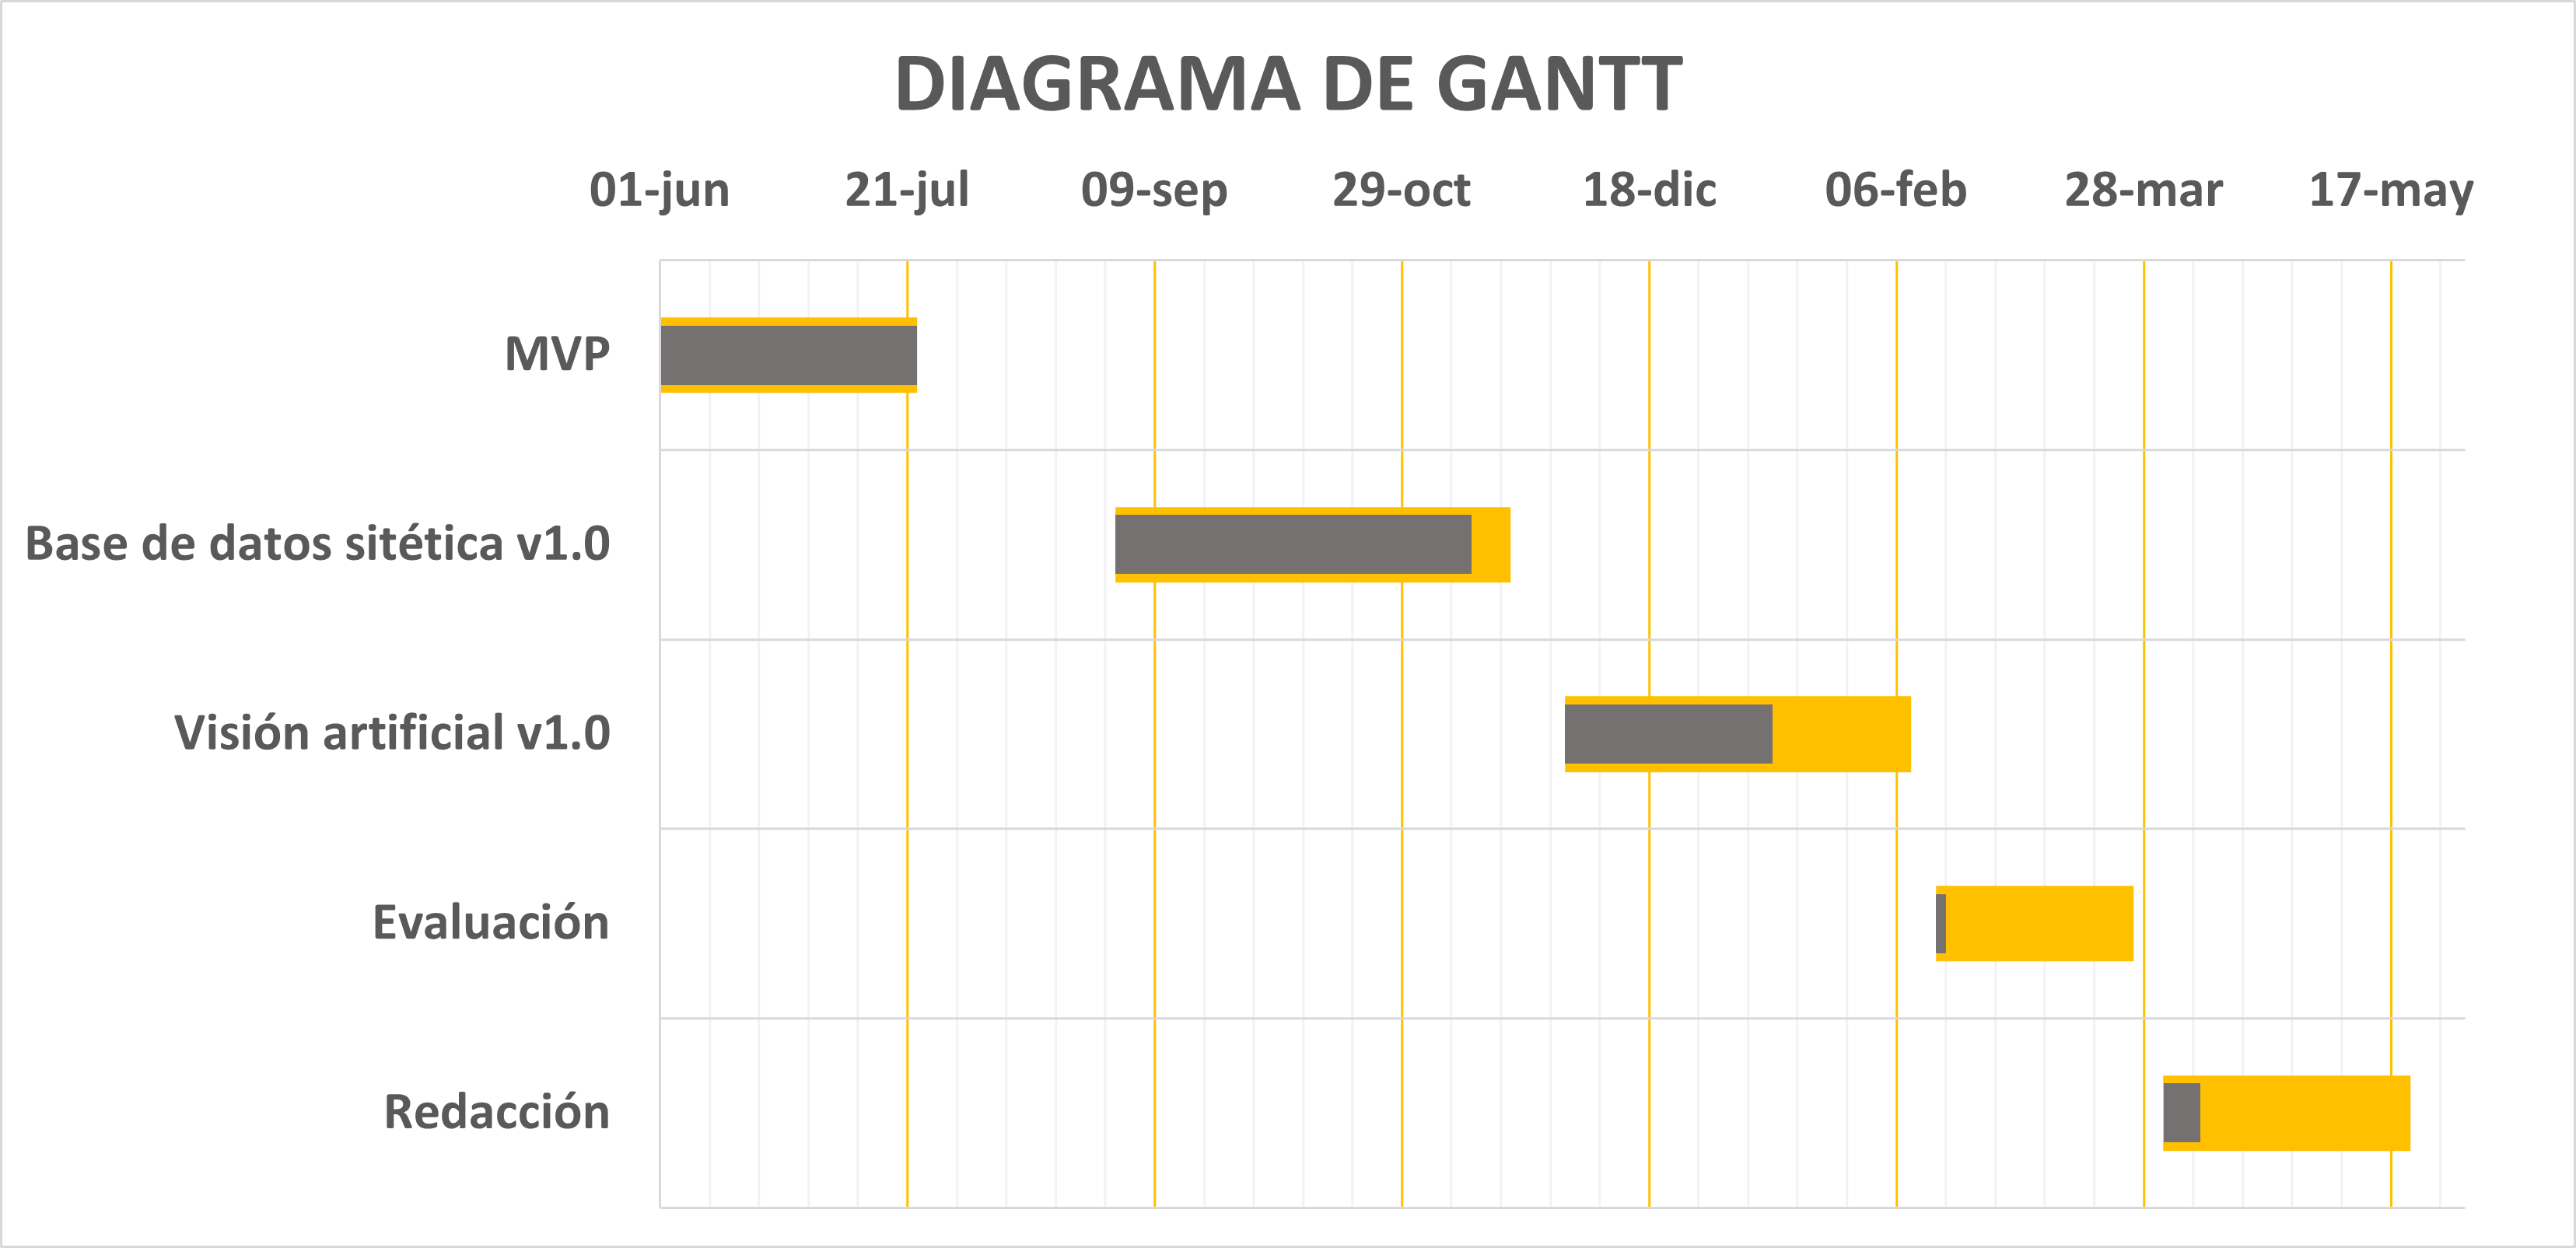
\includegraphics[width=1.0\textwidth]{Metodologia/Diagrama_de_gantt.png}
	\caption{Diagrama de gantt del proyecto}
	\label{chap:Metodología fig:Gantt}
	\vspace{-5pt}
\end{figure}